\section{Управљање процесима}
Процес модел који се користи у MPI-1 имплементацијама користи фиксиран број процеса током MPI рачунања. Ово је концептуално једноставан модел, јер ставља све сложености интеракције са оперативним системом (који мора бити 
укључен у стварање процеса) потпуно изван оквира апликације. Када се изврши \texttt{MPI\_Init}, процеси су покренути и комуникатор \texttt{MPI\_COMM\_WORLD} има коначан број процеса. Они могу међусобно да комуницирају преко комуникатора. Други комуникатори имају своје групе, која је подгрупа \texttt{MPI\_COMM\_WORLD} комуникатора. Динамичнији приступ управљањем процеса пролазилази из \gls{PVM} (\textit{Parallel Virtual Machine}) заједнице, где се процеси покрећу под контролом апликације. Интеркомуникатор служи да повеже две групе процеса. Интеркомуникатори омогућавају природан начин да опишу \textit{spawning} процесе. Интеркомуникатори се могу спојити помоћу функције MPI\_Intercomm\_merge, чије је повратна вредност нови интракомуникатор.

\subsection{\textit{Spawning} процеса}
У MPI-2 имплементацијама, процес се креира помоћу функције \texttt{MPI\_Comm\_spawn}. Кључна предности \texttt{MPI\_Comm\_spawn} су:

\begin{itemize}
	\item Ово је колективна операција над новим процесима.
	\item Нови процеси имају свој властити \texttt{MPI\_COMM\_WORLD}.
	\item Функција \texttt{MPI\_Comm\_parent}, позвана од стране детета процеса, као повратну вредност има интеркомуникатор који садржи децу процеса као локалну групу и родитеље као даљинску групу.
\end{itemize}

\subsection{Пример паралелног копирања}

Једноставан услужни програм који извршава паралелно копирање тако што копира фајл са локалног диска машине на локалне дискове других машина(Листинг 3.13). Са MPI имплементацијом може се на скалабилан начин смањити време извршавања програма. Основни начин слања фајла помоћу MPI-а је користећи функцију  \texttt{MPI\_Bcast} за слање са \textit{root} процеса(слика 3.7). Да би се покренуо програм, потребно је на свакој машини имати извршни фајл. 

\begin{figure}[h!]
  \centering
      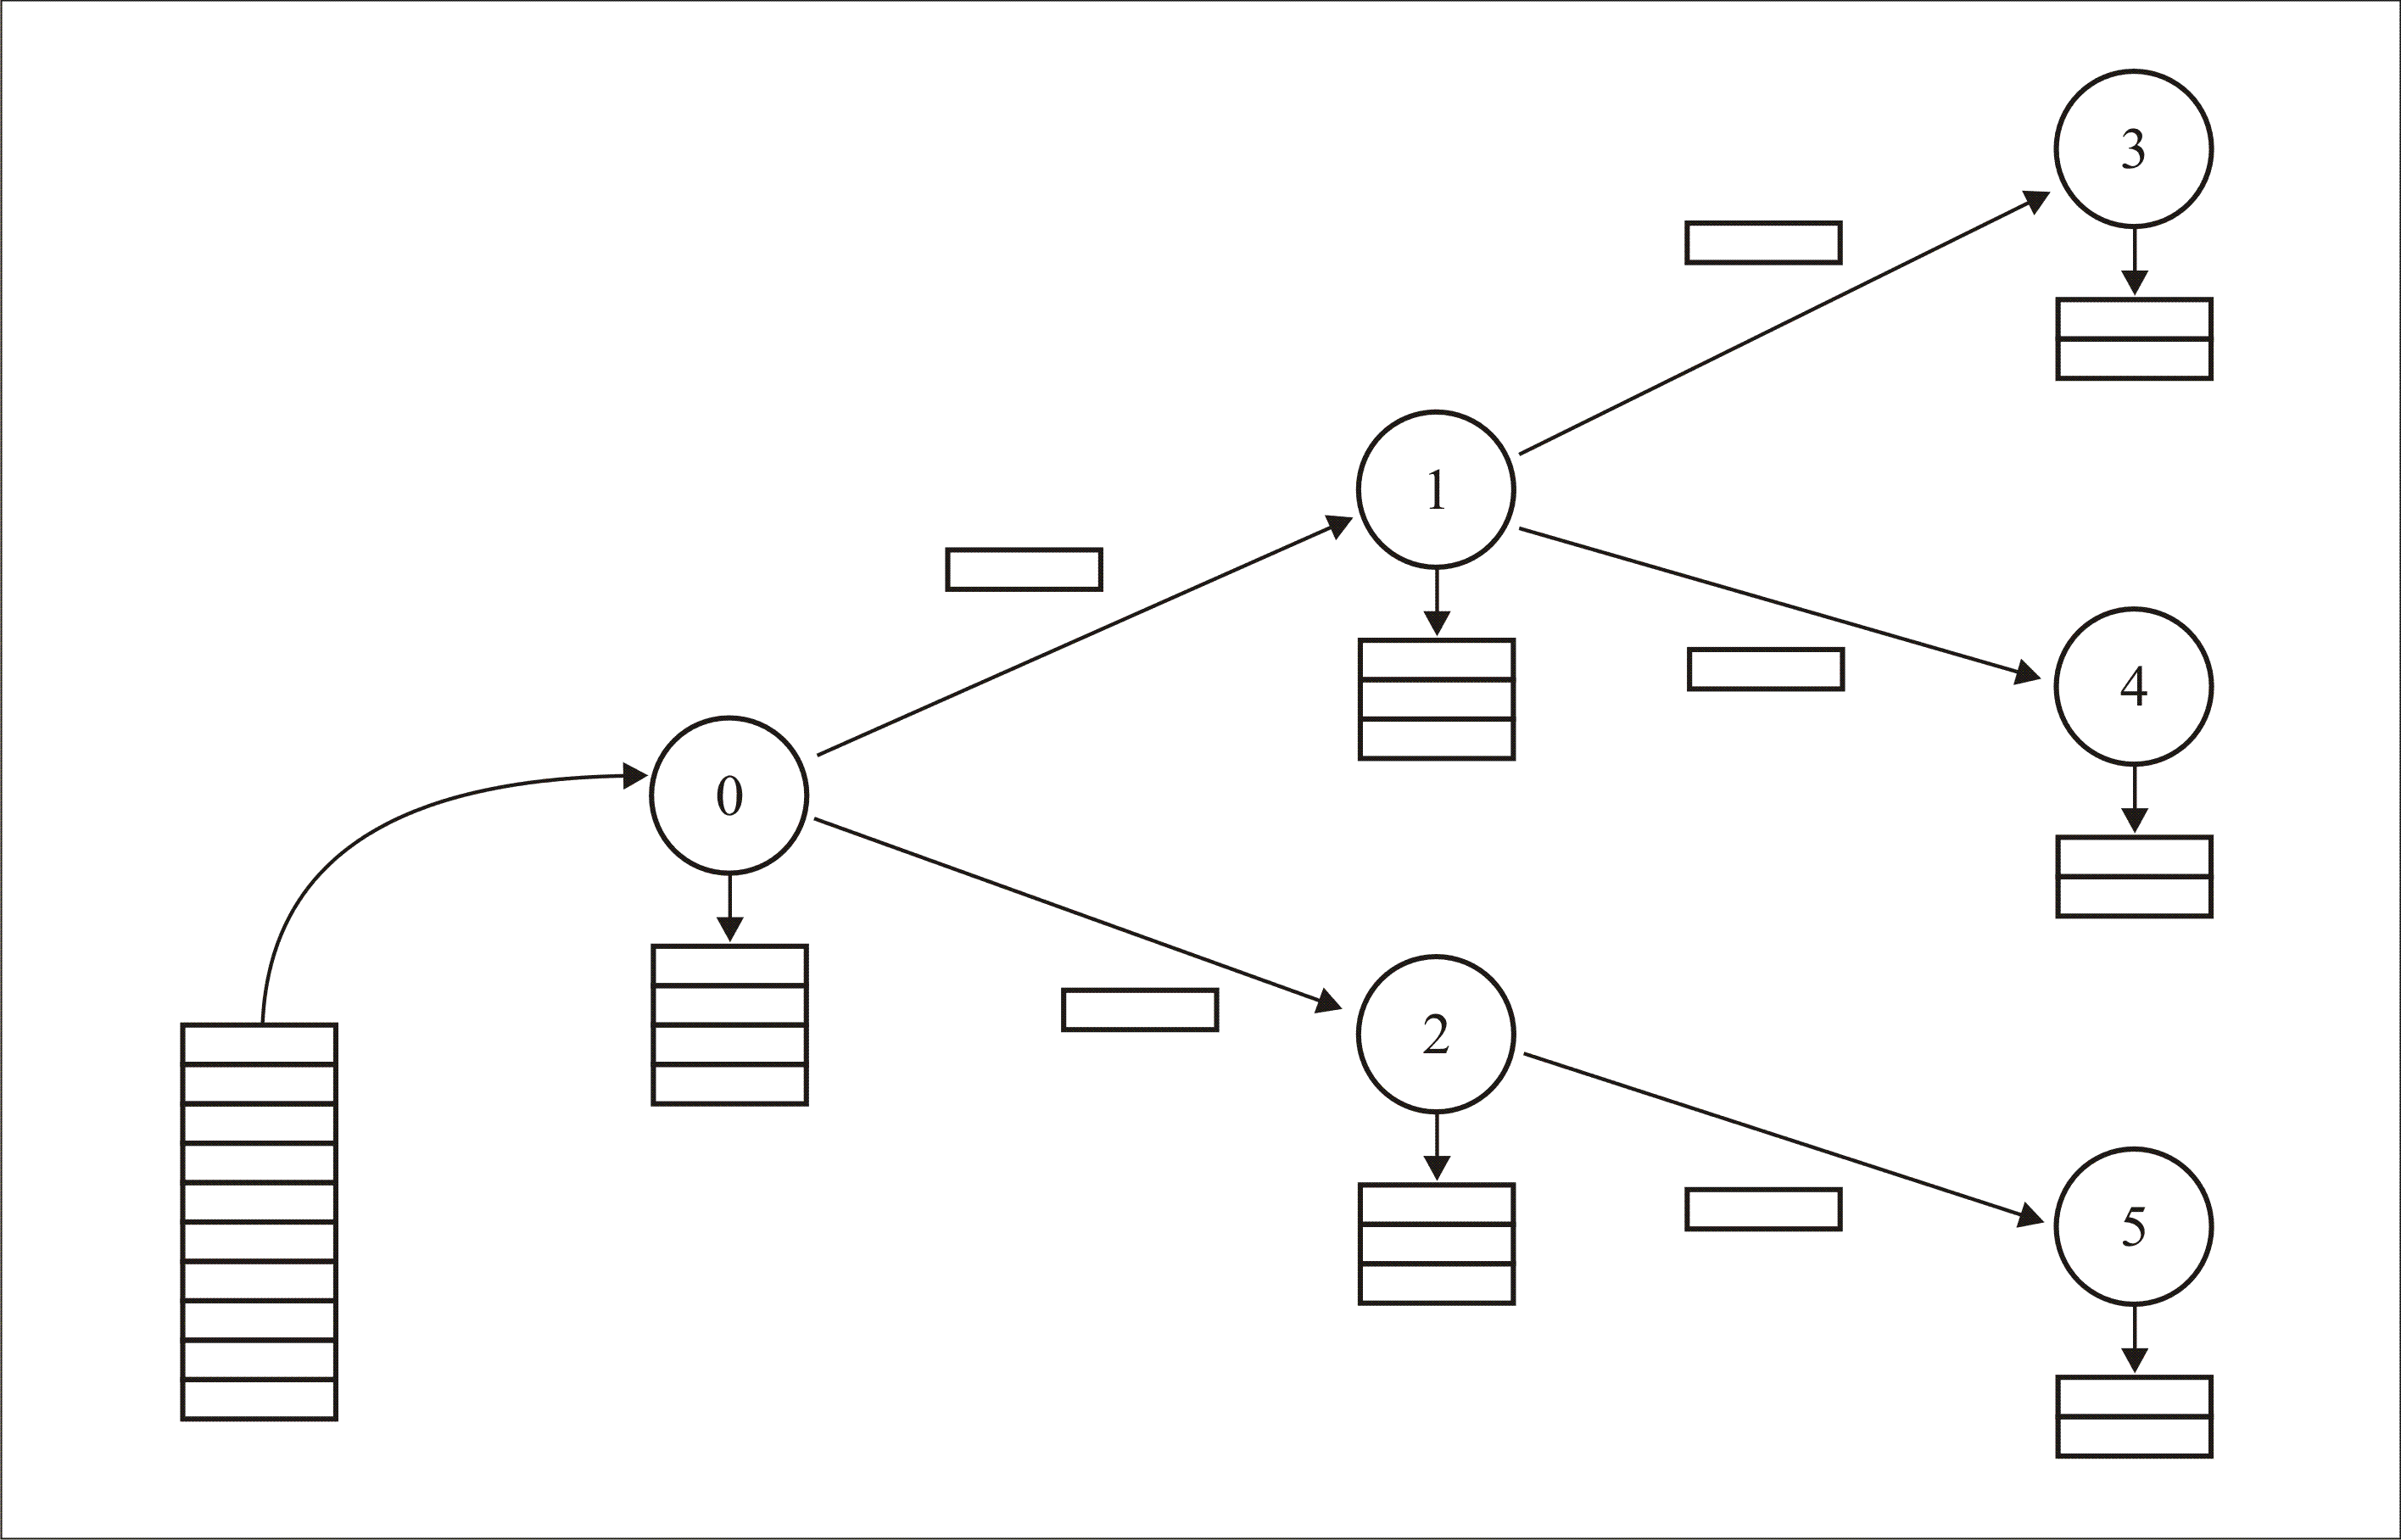
\includegraphics[width=0.5\textwidth]{slike/bcast.png}
  \caption{MPI remote}
\end{figure}

Процес са рангом 0 чита фајл, а затим користећи \texttt{MPI\_Bcast} шаље блок по блок фајла другим процесима. Овај начин садржи 3 облика паралелизма:

\begin{itemize}
	\item Сви процеси извршавају паралелне улазно/излазне операције са фајлом.
	\item Већи део слања порука између процеса се одвија паралелно.
	\item Подела фајла у блокове се одвија у \textit{pipeline} паралелизму.
\end{itemize}

Први део програма је парсирање листе свих машина на које је потребно ископирати фајл, а затим и креирање празног фајла на тим машинама. Функција makehostlist парсира први аргумент и штампа списак машина у фајл чији је назив прослеђен као други аргумент. Број машина је повратна вредност ове функције. 

\begin{verbatim}
makehostlist( argv[1], "targets", &num_hosts );
\end{verbatim}

Да би сви процеси знали име фајла у коме се налази списак машина, потребно је да се назив фајла проследи функцији која покреће нове процесе \texttt{MPI\_Comm\_spawn} помоћу инфо објекта. Креира се инфо објекат који садржи \zn targets" као вредност резервисаног кључа. Овај инфо кључ једноставно говори функцији \texttt{MPI\_Comm\_spawn} да погледа фајл  \zn targets" за више информација. 

\begin{lstlisting}[style=nonumbers,frame=single,language=C, caption= MPI програм за паралелно копирање]
#include "mpi.h"
#include <stdio.h>
#include <sys/types.h>
#include <sys/stat.h>
#include <fcntl.h>
#define BUFSIZE 256*1024
#define CMDSIZE 80

int main( int argc, char *argv[] )
{
	int	num_hosts, mystatus, allstatus, done, numread;
	int	infd, outfd;
	char utfilename[MAXPATHLEN], controlmsg[CMDSIZE];
	char buf[BUFSIZE];
	char soft_limit[20];
	MPI_Info hostinfo;
	MPI_Comm pcpslaves, all_processes;
	MPI_Init( &argc, &argv );
	makehostlist( argv[1], "targets", &num_hosts );
	MPI_Info_create( &hostinfo );
	MPI_Info_set( hostinfo, "file", "targets" );
	sprintf( soft_limit, "0:%d", num_hosts );
	MPI_Info_set( hostinfo, "soft", soft_limit );
	MPI_Comm_spawn( "pcp_slave", MPI_ARGV_NULL, num_hosts,
	hostinfo, 0, MPI_COMM_SELF, &pcpslaves,
	MPI_ERRCODES_IGNORE );
	MPI_Info_free( &hostinfo );
	MPI_Intercomm_merge( pcpslaves, 0, &all-processes );
	strcpy( outfilename, argv[3] );
	if ( (infd = open( argv[2], O_RDONLY ) ) == -1 )
	{
		fprintf( stderr, "input %s does not exist\n", argv[2] );
		sprintf( controlmsg, "exit" );
		MPI_Bcast( controlmsg, CMDSIZE, MPI_CHAR, 0, all_processes );
		MPI_Finalize();
		return -1 ;
	}
	else
	{
		sprintf( controlmsg, "ready" );
		MPI_Bcast( controlmsg, CMDSIZE, MPI_CHAR, 0, all_processes );
	}
	MPI_Bcast( outfilename, MAXPATHLEN, MPI_CHAR, 0,
	all_processes );
	if ( (outfd = open( outfilename, O_CREAT|O_WRONLY|O_TRUNC,
	S_IRWXU ) ) == -1 )
	{
		mystatus = -1;
	}
	else
	{
		mystatus = 0;
	}
	MPI_Allreduce( &mystatus, &allstatus, 1, MPI_INT, MPI_MIN,
	all_processes );
	if ( allstatus == -1 )
	{
		fprintf( stderr, "Output file %s could not be opened\n",
		outfilename );
		MPI_Finalize();
		return 1 ;
	}
	/* at this point all files have been successfully opened */
	done = 0;
	while (!done) 
	{
		numread = read( infd, buf, BUFSIZE );
		MPI_Bcast( &numread, 1, MPI_INT, 0, all_processes );
		if ( numread > 0 ) 
		{
			MPI_Bcast( buf, numread, MPI_BYTE, 0, all_processes );
			write( outfd, buf, numread );
		}
		else
		{
			close( outfd );
			done = 1;
		}
	}
	MPI_Comm_free( &pcpslaves );
	MPI_Comm_free( &all_processes );
	MPI_Finalize();
	return 0;
}
\end{lstlisting}

Програм конвертује интеркомуникатор \texttt{pcpslaves} који садржи покренут процес и процесе које је креирала функција \texttt{MPI\_Comm\_spawn} у један заједнички интракомуникатор помоћу \texttt{MPI\_Intercomm\_merge}. Интракомуникатор \textit{all\_processes} се користи као комуникатор између \textit{root} машине и осталих машина. Процеси покушавају отворити улазни фајл, и уколико дође до грешке, шаље се сигнал за прекид рада.

Да би се знало да је сваки процес отворио фајл, користи се \texttt{MPI\_Allreduce} функција са \texttt{MPI\_MIN} операцијом. Уколико било који процес не може да отвори фајл, сви процеси ће то сазнати и позвати 
\texttt{MPI\_Finalize} за прекид рада. Код за дете процес је сличан коду родитеља процеса, с тим што дете процеса мора да позове \texttt{MPI\_Comm\_get\_parent} функцију да успостави контакт са родитељем. Дете процес не обрађује аргументе нити штампа поруке. Родитељ процес затим чита блок по блок фајла и шаље осталим процесима. На крају сви процеси ослобађају интеркомуникатор креиран од стране  \texttt{MPI\_Comm\_spawn} и обједињени интракомуникатор. Главна разлика између \texttt{MPI\_Comm\_spawn} функције и осталих  система за слање порука је природност колективних операција. У MPI имплементацији, група процеса колективно креира другу групу процеса који су међусобно синхронизовани. Тиме се спречавају додатни услови и омогућава неопходна комуникациона инфраструктура.

\chapter{Закључак}     

 Главни недостатак \textit{Lustre} фајл система је компликована инсталација у односу на његову алтернативу NFS. Међутим, уштеда времена у току вршења тестирања је огромна што се никако не сме занемарити. Та предност је нарочито значајна при извршавању обимних математичких операција које захтевају рад са фајловима. MPI-2 стандард са новим функцијама које омогућавају паралелне улазно/излазне операције заједно са \textit{Lustre} фајл системом чине најбољу комбинацију за паралелне програме. Обзиром да је \textit{Lustre} фајл систем доступан бесплатно, да је његов опоравак лакши у случају отказивања чврстог диска и да подржава паралелне операције са фајловима, треба му се дати апсолутна предност у односу на NFS. Једина алтернатива коју \textit{Lustre} тренутно има на тржишту је \textit{PanFS} компаније \textit{Panasas}, који се нешто лакше конфигурише и администрира, али по цену затворености кода и више цене. 

